\subsection{Event distribution varied with time}

In this section, we analysis how many load and drop event happened for each hour.  
\begin{table}[!h]
\caption{Events quantity varied with time}\label{table_event_distribution_with_time}
\centering
\begin{tabular}{l|c|c}
 \hline
 item &drop event quantity &load event quantity \\
  \hline
  total quatity for a week& 2,679,385&2,707,290\\
  maximum of an hour&28,583 &28,130\\
  minmum of an hour&861&918\\
  time of the peak value&2011/11/04 19:00-20:00&2011/11/04 19:00-20:00\\
  time of the valley&2011/11/03 4:00-5:00&2011/11/03 4:00-5:00\\
  \hline
  \end{tabular}
\end{table}

\begin{figure}[!h]
\centering
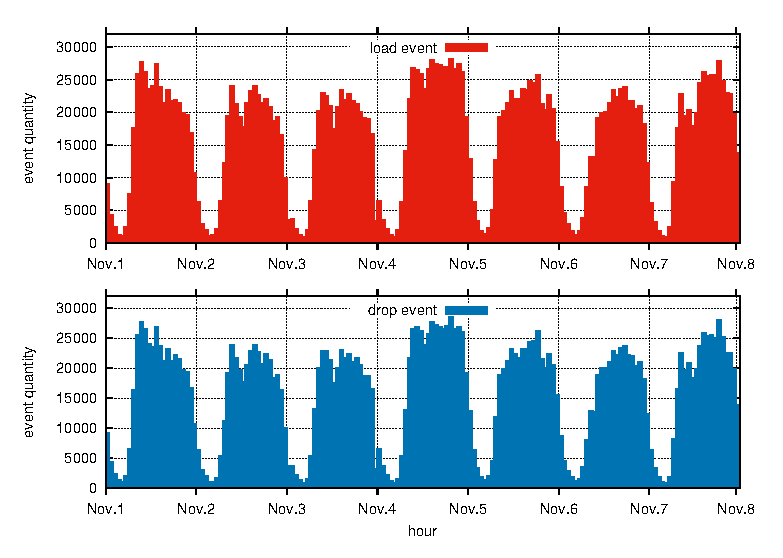
\includegraphics[width=0.5\textwidth]{figures_201103/analysis/event_w_time.eps}\\
\caption{Taxi event varied with time.}\label{figure_event_varied_w_t}
\end{figure}


\begin{figure}[!h]
\centering
\begin{tabular}
[c]{cc}
\epsfysize=1.3in\epsfbox{figures_201103/analysis/hotspots/hotspot_drop_04.eps} &
\epsfysize=1.3in\epsfbox{figures_201103/analysis/hotspots/hotspot_drop_19.eps} \\
(a) drop events at 4:00-5:00 & (b) drop events at 19:00-20:00\\
\epsfysize=1.3in\epsfbox{figures_201103/analysis/hotspots/hotspot_load_04.eps} &
\epsfysize=1.3in\epsfbox{figures_201103/analysis/hotspots/hotspot_load_19.eps} \\
(c) load events at 4:00-5:00 & (d) load events at 19:00-20:00\\
\end{tabular}
\caption{Taxi density for load/drop events in one hour.}\label{figure_taxi_density_for_one_hour}
\end{figure}


\begin{itemize}
  \item For drop and load event, the total event number for a week are very close. \\
  \item The peak and valley occurs in similar time. From the data, we can find that the peak and valley happened at same time, coincidentally.
  \item The maximum event number is much larger than the minimum event number. The quantity of event number changes over time. The curves for the load and drop events follows similar rules. The quantities at the same time range are similar, too.
\end{itemize}

The analysis results fit with our daily experience: (1) the amount of passengers decreases early in the morning, (2) the load event quantity equilibrates with the drop event quantity, and (3) the event quantity at certain time shows certain regularity. 

